% !TEX TS-program = pdflatex
% !TEX encoding = UTF-8 Unicode

% This is a simple template for a LaTeX document using the "article" class.
% See "book", "report", "letter" for other types of document.

\documentclass[11pt]{article} % use larger type; default would be 10pt

\usepackage[utf8]{inputenc} % set input encoding (not needed with XeLaTeX)

%%% PAGE DIMENSIONS
\usepackage{geometry} % to change the page dimensions
\geometry{a4paper} % or letterpaper (US) or a5paper or....

\usepackage{graphicx} % support the \includegraphics command and options

\usepackage{amssymb}
\usepackage{amsmath}
%%% PACKAGES
\usepackage{booktabs} % for much better looking tables
\usepackage{array} % for better arrays (eg matrices) in maths
\usepackage{paralist} % very flexible & customisable lists (eg. enumerate/itemize, etc.)
\usepackage{verbatim} % adds environment for commenting out blocks of text & for better verbatim
\usepackage{subfig} % make it possible to include more than one captioned figure/table in a single float
% These packages are all incorporated in the memoir class to one degree or another...

%%% HEADERS & FOOTERS
\usepackage{fancyhdr} % This should be set AFTER setting up the page geometry
\pagestyle{fancy} % options: empty , plain , fancy
\renewcommand{\headrulewidth}{0pt} % customise the layout...
\lhead{}\chead{}\rhead{}
\lfoot{}\cfoot{\thepage}\rfoot{}

%%% SECTION TITLE APPEARANCE
\usepackage{sectsty}
\allsectionsfont{\sffamily\mdseries\upshape} % (See the fntguide.pdf for font help)
% (This matches ConTeXt defaults)

%%% ToC (table of contents) APPEARANCE
\usepackage[nottoc,notlof,notlot]{tocbibind} % Put the bibliography in the ToC
\usepackage[titles,subfigure]{tocloft} % Alter the style of the Table of Contents
\renewcommand{\cftsecfont}{\rmfamily\mdseries\upshape}
\renewcommand{\cftsecpagefont}{\rmfamily\mdseries\upshape} % No bold!

\usepackage{amsmath}
\usepackage{graphicx}
\graphicspath{ {./pings/} }
\DeclareMathOperator*{\argmax}{arg\,max}
\DeclareMathOperator*{\argmin}{arg\,min}

\newcount\colveccount
\newcommand*\colvec[1]{
        \global\colveccount#1
        \begin{pmatrix}
        \colvecnext
}
\def\colvecnext#1{
        #1
        \global\advance\colveccount-1
        \ifnum\colveccount>0
                \\
                \expandafter\colvecnext
        \else
                \end{pmatrix}
        \fi
}

%%% END Article customizations

%%% The "real" document content comes below...

\title{Micro HW4}
\author{Michael B. Nattinger\footnote{I worked on this assignment with my study group: Alex von Hafften, Andrew Smith, Ryan Mather, and Tyler Welch. I have also discussed problem(s) with Emily Case, Sarah Bass, and Danny Edgel.}}

%\date{} % Activate to display a given date or no date (if empty),
         % otherwise the current date is printed 

\begin{document}
\maketitle

\section{Question 1}
\subsection{Part A} %note: s here should now be a mapping so I need to change this
$N = \{ A,B \}, a_i = v_i \in V, \theta_i = b_i \in \Theta, S_i: V \rightarrow \Theta, \\u_i(b_i,b_{-i}|v_i) = \begin{cases} p(v_i - b_i) + q(v_i - b_{-i}) +(1-p-q)v_i | b_{i}>b_{-i} \\ (1-p-q)( - b_i) | b_{i}<b_{-i} \\ (1/2)(v_i - b_i) | b_{i}=b_{-i} \end{cases}$
\subsection{Part B}
\begin{align*}
u_i(b_i,v_j|v_i) &= (p(v_i - b_i) + q(v_i - b(v_j)) + (1-p-q)v_i)P(b_i>b(v_j))\\
&+ (1-p-q)(- b_i)P(b_i<b(v_j)) + (1/2)(v_i - b_i)P(b_i=b(v_j))\\
\Rightarrow U_i(b_i|v_i) &= \int_0^1 u_i(b_i,v_j|v_i)f(v_j)dv_j\\
&=  \int_0^1(p(v_i - b_i) + q(v_i - b(v_j))+ (1-p-q)v_i)1\{b_i>b(v_j)\}\\
&+ (1-p-q)(- b_i)1\{b_i<b(v_j)\} + (1/2)(v_i - b_i)1\{b_i=b(v_j)\}dv_j\\
&=\int_{0}^{b^{-1}(b_i)}p(v_i - b_i) + q(v_i - b(v_j))+ (1-p-q)v_i dv_j +(1-p-q)( - b_i)(1-b^{-1}(b_i))\\
&= b^{-1}(b_i)(p(v_i - b_i)+ (1-p-q)v_i) \\&+ \int_{0}^{b^{-1}(b_i)}q(v_i - b(v_j))dv_j + (1-p-q)( - b_i)(1-b^{-1}(b_i))
\end{align*}
\subsection{Part C}
Taking FOCs with repect to $b_i$,
\begin{align*}
%u_i(b(v_i)|v_i) &= (p(v_i - b(v_i)) + q(v_i - b(v_j)))P(b(v_i)>b(v_j))\\
%&+ (1-p-q)(v_i - b(v_i))P(b(v_i)<b(v_j)) + (1/2)(v_i - b(v_i))P(b(v_i)=b(v_j))\\
%&= (p(v_i - b(v_i)) + q(v_i - b(v_j)))P(v_i>v_j) + (1-p-q)(v_i - b(v_i))P(v_i<v_j)\\
%&=(p(v_i - b(v_i)) + q(v_i - b(v_j)))v_i + (1-p-q)(v_i - b(v_i))(1-v_i).\\
%\Rightarrow u
%u_i(v_i) &= \int_0^1(p(v_i - b(v_i)) + q(v_i - b(v_j)))1\{b(v_i)>b(v_j)\}\\
%&+ (1-p-q)(v_i - b(v_i))1\{b(v_i)<b(v_j)\} + (1/2)(v_i - b_i)1\{b(v_i)=b(v_j)\}dv_j\\
%&= \int_0^{v_i}(p(v_i - b(v_i)) + q(v_i - b(v_j))) dv_j+ \int_{v_i}^1(1-p-q)(v_i - b(v_i))dv_j
& (1-p-q)(1-b^{-1}(b_i)) + (1-p-q)( - b_i)\frac{1}{b'(b^{-1}(b_i))} + b^{-1}(b_i)p\\&= \frac{1}{b'(b^{-1}(b_i))}(p(v_i - b_i) + (1-p-q)v_i) + q(v_i - b(b^{-1}(b_i)))\frac{1}{b'(b^{-1}(b_i))}
\end{align*}
\begin{align*}
\Rightarrow b'(v_i) (1-p-q)(1-v_i) + (1-p-q) ( - b(v_i)) + b'(v_i) v_i p &= p(v_i - b(v_i)) + q(v_i - b(v_i)) + (1-p-q)v_i
\end{align*}
Now, assume $b$ is affine: $b(x) = ax+c$.
\begin{align*}
\Rightarrow a(1-p-q)(1-v_i) + (1-p-q) (- av_i - c) +av_i p &= p(v_i - av_i - c) + q(v_i - av_i - c) + (1-p-q)v_i
%(1-p-q)(1-v_i) + (1-p-q)(v_i - b_i)\frac{1}{a} &= p(v_i - av_i - c) + q(v_i - av_i - c)
%u_i(b(v_i)|v_i) &=(p(v_i - av_i -c)) + q(v_i - av_j-c))v_i + (1-p-q)(v_i - av_i - c)(1-v_i)\\
%&= pv_i^2 - pav_i^2 - pcv_i + qv_i^2 -qav_jv_i - qcv_i + (1-p-q)v_i - a(1-p-q)v_i - (1-p-q)c - (1-p-q)v_i^2
%u_i(v_i) &=\int_0^{v_i}(p(v_i - av_i - c) + q(v_i - av_j - c)) dv_j+ \int_{v_i}^1(1-p-q)(v_i - av_i - c)dv_j\\
%&= p(1-a)v_i^2 - pcv_i + qv_i^2 - cv_i -aqv_i^2/2 + (1-p-q)((1-a)v_i - c)(1-v_i)\\
%&= (p(1-a) + q(1-a/2))v_i^2
\end{align*}
This must hold $\forall v_i$ so it must hold for $v_i=0,v_i=1:$
\begin{align*}
v_i = 1 \Rightarrow (1-p-q)(-a-c) + ap &= (p+q)(1-a-c) +(1-p-q) \\
%\Rightarrow (1-p-q) &= ap + q\\
%\Rightarrow a &= \frac{1-p-2q}{p}\\
v_i = 0 \Rightarrow  (1-p-q)(a - c) &= -(p + q)c\\
\Rightarrow c&= \frac{p+q-1}{8p^2 + 14pq -8p + 6q^2 - 7q +2}\\
\Rightarrow a&= \frac{1}{4p + 3q -2}
%\Rightarrow c &= \frac{(1-p-q)\left(\frac{1-p-2q}{p}\right)}{(1-p-q) -\left(\frac{1-p-2q}{p}\right)(p+q)}
\end{align*}
Therefore, the symmetric bayesian nash equilibrium with a linear response function is to bid using the formula:
\begin{align}
b(v) &= \left(  \frac{1}{4p + 3q -2}\right)v + \frac{p+q-1}{8p^2 + 14pq -8p + 6q^2 - 7q +2} \label{eqn:bne}
\end{align}
\subsection{Part D}
From (\ref{eqn:bne}) we can see the following:
\begin{itemize}
\item As $p\rightarrow 1$ the intercept goes to 0 and the slope term goes to $\frac{1}{2}$.
\item As $q\rightarrow 1$ (and $p\rightarrow0$) the intercept again goes to 0 and the slope term now goes to $1$.
\item As $q\rightarrow \frac{1}{2}$ (and $p\rightarrow0$), the intercept goes to $+\infty$ and the slope goes to $-2$.
\end{itemize}
\section{Question 2}
\subsection{Part A}
First, consider the case where $\beta<0.$ Then, none of the strategies are strictly dominated and pure strategy nash equilibria exist at $(A,B)$,$(B,A)$ and we can find a mixed strategy nash equilibrium: $(\frac{-\beta}{1-\beta}A + \frac{1}{1-\beta}B ,\frac{-\beta}{1-\beta}A + \frac{1}{1-\beta}B)$.

Next, consider $\beta = 0.$ Then, pure strategy nash equilibria are now at $(A,B),(B,A)$, however the mixing equilibrium no longer exists.

Finally, consider $\beta>0$. Then, a pure strategy nash equilibria exists at $(B,B)$ and no mixed strategy exists. 
\subsection{Part B}
$\beta_i \in \beta, \theta_i \in \Theta = \{ A,B\}, S_i: \beta \rightarrow \Theta$.
\begin{align*}
u(\theta_i,\theta_j|\beta_i) &= \begin{cases} 1,\theta_i = \theta_j = A \\ 0,\theta_i = A, \theta_j = B \\ 2,\theta_i = B, \theta_j = A\\ \beta,\theta_i = \theta_j = B \end{cases}\\
U(\theta_i|\beta_i) &= \begin{cases} P(\theta_j = A), \theta_i = A \\ 2P(\theta_j = A) +\beta_i(1-P(\theta_j=A)) , \theta_i=B\end{cases} 
\end{align*}

Since the choice is discrete, we know that there is a unique point $\beta^{*}$ such that $\beta_i<\beta^{*}\iff\theta_i = A$. By symmetry this implies that $\beta^{*}$ satisfies the following equation (1 variable in 1 unknown):
\begin{align*}
F(\beta^{*})&=2F(\beta^{*}) + \beta^{*}(1-F(\beta^{*}))
\end{align*}

Then, $\theta_i(\beta_i) = \begin{cases} A, \beta_i<\beta^{*} \\ B, \beta_i\geq\beta^{*} \end{cases}$ is the bayesian nash equilibrium.
\subsection{Part C}
Depending on the values of $\beta_1,\beta_2,$ no correlated equilibria can occur as B strictly dominates A for both players 1 and 2. %correlated equilibria can be achieved for   $\{(A,A),(B,A),(A,B),(B,B)\}$.
\subsection{Part D}
For the equilibrium to hold, the expected utility of abiding by the equilibrium must be at least the utility of diverging.

If person  A is told to play A, they will play A if $\frac{1-2p}{1-p}(1) + \frac{p}{1-p}(0)\geq \frac{1-2p}{1-p}(2) + \frac{p}{1-p}(\beta_1)$ and if told to play B will do so if $2>1$. These conditions (really only the first is actually useful) imply that $\beta_1 \leq \frac{2p-1}{p}$. Similar conditions for person B imply that $\beta_2 \leq \frac{2p-1}{p}$. For very small levels of $p$, each $\beta_i$ must be below a critical point which goes to $-\infty$ in the limit as $p\rightarrow 0$ for the equilibrium to be supported. As $p$ increases, the critical level below which each $\beta_i$ must  remain for the equilibrium to be supported increases, eventually approaching $0$ as $p\rightarrow 1/2$.

If we restrict each $\beta_i>0$, then no equilibrium can be supported (as $p\leq\frac{1}{2}$). Thus, this equilibrium is not included in Part C.
\section{Question 3}
All theorists smell either nine or 10 bad breaths. When the first elevator comes, someone would only come on if they smelled no other bad breaths. Nobody gets on, so at least two have bad breath. When the secoond elevator comes, someone would only come on if they smelled one other person with bad breath. Nobody gets on, so at least three have bad breath. When the fourth elevator comes, the process repeats again, as it does for elevators 5, 6, 7, 8, and 9. When the tenth elevator comes, someone would only get on if they smelled 9 other people with bad breath. 10 people do smell 9 other people with bad breath, so all 10 people with bad breath gets on the elevator.
\section{Question 4}
\subsection{Part A}
We will take the hint as given and observe that, in all SPE a player's choice depends only on the number of steps he has left and the opponent's steps. The column labels in the below table represent the location of the player about to move, and the column labels represent the number of steps the opponent has left. The table will show the optimal move, and we can work backwards to determine the optimal movement of the players.
\begin{center}
\begin{tabular}{r | c c c c c c }
& 6&5&4&3&2&1\\
\hline
6 &(II) & (I) & (I) & (I) &(I) &(I)\\
5&(II) & (III) & (III) & (I) &(I) &(I)\\
4&(II) & (II) &(II) & (I) &(I) &(I)\\
3&(II) & (II) & (II) &(IV)&(IV)&(IV)\\
2 &(II) &(II) & (II) &(III)&(III)&(III)\\
1&(II)&(II)&(II)&(II)&(II)&(II)
\end{tabular}
\end{center}
For the bottom right (3 by 3) corner of the table, either player will win positive payoff with their next move, so if the player currently playing does not move to win then the other player will move to win in the next period. Thus, the current player will move to win and will receive a positive payoff. In the bottom left corner the current player should move forward by just one move as the other player has no ability to win in the next period, and because moving one step and then two steps is cheaper than moving three steps at once (and similarly moving one step at a time twice is cheaper than moving two steps immediately). The top-right corner is a losing position for the current player- they cannot jump into a winning position (as the other player can immediately win in the next period) and such are best off cutting their losses and not moving. Now, of more interest is the upper-right corner.

If the current player finds themselves at (4,4), then they should move forward by one space. The other player will see (4,3) when they move, which is a losing position, so the current player wins by moving forward one space. Similarly, if the current player finds themselves at (5,4) or (5,5), then they should move forward by 2 spaces. The other player will see (4,3) or (5,3) in the next turn, always a losing position. Moreover, the current player should move one spot forward at (4,6) and (4,5) as it moves them into a winning position.   

If the current player finds themselves at (6,5) or (6,4), they should give up - it is too costly to try to jump ahead (as moving up by 3 and then by one 3 times would result in a win, but would cost more than it wins. Due to this, a player finding themselves at (6,6) or (5,6) should move up by one as they can force the opponent into losing positions.

Now that we have formed our table of best responses, above, we can summarize: The player that wins the coin toss and moves first will move forward, one space at a time, every turn. The other player will deduce from the very beginning that they have lost, as it is too costly to jump ahead back into a winning position, and so they will cut their losses by not moving.

Therefore, the subgame perfect equilibria is for the player that can move first to move forwards, one turn at a time, six times, and for the other player to not move.
\subsection{Part B}
For Arthur, in either case he is best off by moving forwards one step at a time as it is the most efficient way to move towards the prize in the game. The other 'jump' options serve rather the purpose of 'jumping' over opposition and into winning positions in the competitive case, and the 'halt' option serves the purpose of cutting losses if one finds themselves in a winning position. Neither of these options are useful in the non-competitive case as they provide less payoff than moving forwards one step at a time.
\section{Question 5} % induction
Let two players, A and B, be in a finite two-player zero-sum game of perfect information. We will show that there is a unique subgame perfect equilibrium payoff vector by induction. Without loss of generality, we will represent all games in their extensive form.

Let the game have one round - that is, one choice for one of the players to make. Then, the player making the choice, which without loss of generality we will call player A, can see the possible outcomes they have choice over and will choose the best payoff for themselves. If there were multiple non-unique SPE payoff vectors, then this would immediately be a contradiction as player A would only choose the action(s) with the highest payoff, and not any other actions. If there is a tie, this does not affect the uniqueness of the SPE payoff vector. Furthermore, as the game is zero-sum, player B's payoff from player A's choice is exactly the opposite of player A's payoff and so will also be unique. Therefore, in this game there is a unique SPE payoff vector.

Now, assume that games of size $k$ have a unique SPE payoff vector. Then, consider a game of size $k+1$ and let player A choose in the first action node. Then,   Person B is choosing at the nodes in the second stage. They have a unique SPE payoff vector at each of these nodes, and will choose an action to attain such a payoff. Then, player A has perfect information and knows these payoffs for each second-stage node. Player A will then choose the action which attains the highest payoff for them. As in the base case, there can only be exact ties as player A will not choose any actions which attain less than their maximum payoff from the options they have, and due to the zero-sum nature of the game, player B will attain exactly the opposite level of payoff as player A. Therefore, in this case there is a unique SPE payoff vector, and by induction this is also the case for any finite two-player zero-sum game of perfect information.
\section{Question 6}
\subsection{Part A}
Firm $i$ takes the actions of the other firm as given and maximizes profits. $N = \{A,B\}$, $S_i = p_i \in (0,1)$, $u_i = \pi_i = D_ip_i$.
\begin{align*}
\max_{p_i} D_ip_i &= \max_{p_i} (d - p_i + \alpha p_j)p_i\\
&= \max_{p_i} dp_i - p_i^2 + \alpha p_ip_j\\
\frac{\partial \pi_i}{\partial p_i} = 0 \Rightarrow p_i &= \frac{d + \alpha p_j}{2}
\end{align*}
We can assume that the other firm is also taking the actions of the other firm as given and optimizing, giving us the following expression:
\begin{align*}
p_i &= \frac{d + \alpha \left(\frac{d + \alpha p_i}{2} \right)}{2}\\
\Rightarrow p_i &= \frac{d}{2} + \frac{\alpha d}{4} + \frac{\alpha}{4}p_i\\
\Rightarrow p_i &= \frac{4}{4-\alpha}\left(\frac{d}{2} + \frac{\alpha d}{4}\right)\\
\Rightarrow p_i &= d\frac{2+\alpha}{(2-\alpha)(2+\alpha)}\\
\Rightarrow p_i &= \frac{d}{2-\alpha}
\end{align*}

Therefore, $p_A = p_B = \frac{d}{2-\alpha}$ is the nash equilibrium.
\subsection{Part B}
Firm A looks forward, calculates Firm B's optimal response to any price level Firm A sets, then chooses their own price level to set that will maximize their own profits given Firm B's response.  We have already calculated the best response for firm B to the price set by firm A as a sub-result in Part A, $p_B =  \frac{d + \alpha p_A}{2}$. 

Firm A then solves the following optimization problem:
\begin{align*}
&\max_{p_A} dp_A - p_A^2 + \alpha p_A\left(  \frac{d + \alpha p_A}{2}\right)\\
&\max_{p_A} dp_A - p_A^2 + \frac{\alpha^2 p_A^2}{2} + \frac{\alpha p_A d}{2}\\
\frac{\partial \pi_A}{\partial p_A} =0 &\Rightarrow 2 p_A = d + \alpha^2 p_A + \frac{\alpha d}{2}\\
&\Rightarrow p_A = \frac{d\left(1 + \frac{\alpha }{2}\right)}{2 - \alpha^2} = \frac{d(2+\alpha)}{2(2-\alpha^2)}\\
&\Rightarrow p_B = \frac{d}{2}\left(1 + \alpha \frac{(2+\alpha)}{2(2-\alpha^2)} \right)%\frac{d+\alpha\left( \frac{d\left(1 + \frac{\alpha }{2}\right)}{2 - \alpha^2} \right)}{2}
\end{align*}
\subsection{Part C}

\begin{center}
\begin{tabular}{r | c c}
& Part A & Part B \\
\hline
A price & $\frac{d}{2-\alpha}$ & $\frac{d(2+\alpha)}{2(2-\alpha^2)}$ \\
B price & $\frac{d}{2-\alpha}$ & $\frac{d}{2}\left(1 + \alpha \frac{(2+\alpha)}{2(2-\alpha^2)} \right)$ \\
A profits & $\frac{d^2}{(2-\alpha)^2} $ & $\frac{d^2(\alpha+2)^2(3-\alpha^2)}{16 (2 - \alpha^2)^2}$ \\
B profits & $\frac{d^2}{(2-\alpha)^2}$ & $\frac{d^2}{4}\left(1 + \alpha \frac{(2+\alpha)}{2(2-\alpha^2)} \right)$ \\
Total profits &$\frac{2d^2}{(2-\alpha)^2}$ &$ \frac{d^2(\alpha^4 - 8\alpha^3 - 13\alpha^2 +20\alpha + 28)}{16(2 - \alpha^2)^2}$
\end{tabular}
\end{center}

The table above shows the analytical form of the solution to the problems in parts A and B. They are, however, hard to compare in the exact solution so below I have included figures showing the solution results numerically across a grid of $d$ values for $\alpha \in \{ 0.3,0.6,0.9\}$.

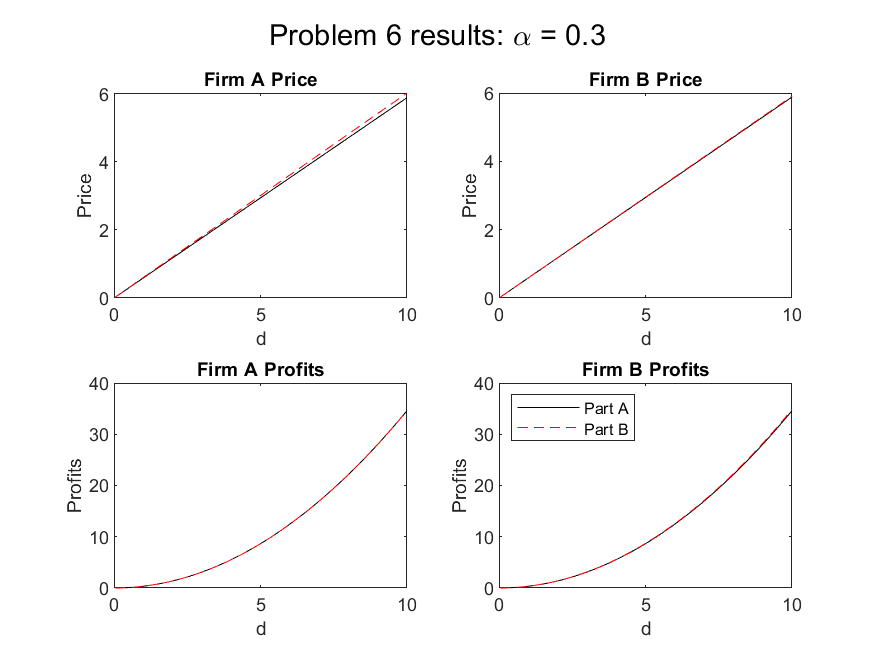
\includegraphics{fig1}

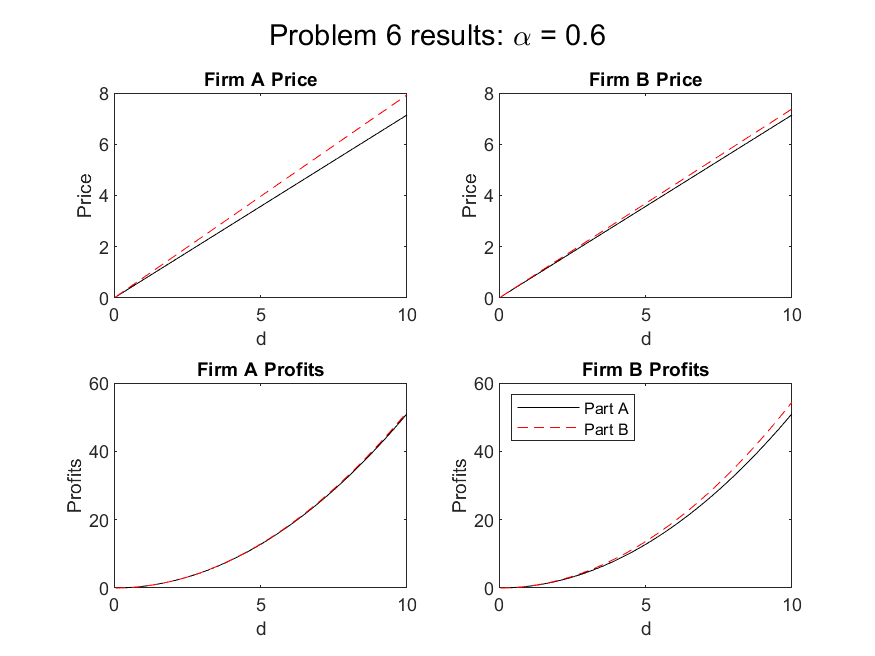
\includegraphics{fig2}

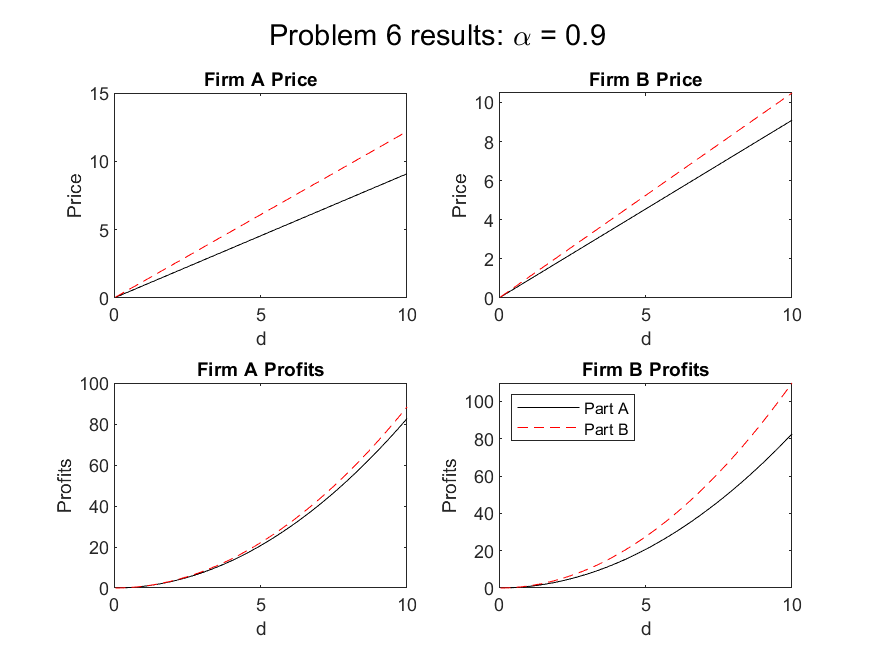
\includegraphics{fig3}

The above figures tell a consistent story. Compared to the base case in part A, in part B the firm that moves second (Firm B) has an incentive to raise their prices, as Firm A cannot react after they originally set their price level. Firm A anticipates this and raises their prices accordingly. The net effect is Firm B raising their profits, which we would expect. It also turns out that Firm A also ends up raising their profits on net, slightly, as the increased revenue per quantity sold raises their profits by slightly more than the reduction in quantity sold decreases their profits.
\end{document}
